\documentclass[12pt]{article}

\usepackage{amssymb,amsmath,amsfonts, booktabs, dsfont, eurosym,float,geometry,ulem,graphicx,caption,color,setspace,sectsty,comment,footmisc,caption,multicol, multirow, natbib, pdflscape,array,hyperref}
\bibliographystyle{rusnat}
\bibliography{citations}

\normalem

\geometry{left=1.0in,right=1.0in,top=1.0in,bottom=1.0in}

\begin{document}



\begin{titlepage}
\title{Arjun Shanmugam's Senior Thesis}
\author{Arjun Shanmugam}
\date{\today}
\maketitle
\begin{abstract}
\noindent Placeholder\\

\bigskip
\end{abstract}
\setcounter{page}{0}
\thispagestyle{empty}
\end{titlepage}
\pagebreak \newpage

\doublespacing

\section{Introduction} \label{sec:introduction}
\bibliography{writing/paper/citations}
\subsection{Literature Review}

\section{Institutional Context}
    \subsection{Eviction in Massachusetts}
        \subsubsection{The Massachusetts Housing Court}
        \subsubsection{The Eviction Process}
    \subsection{Property Tax Assessment}
        \subsubsection{The Property Value Assessment Process}
    \subsection{Zestimates}
        \subsubsection{How Are Zestimates Produced?}
        \subsubsection{Reliability}
\section{Data} \label{sec:data}
    \begin{landscape}
    \subsection{Evictions Data}
        \begin{figure}[H]
            \centering
            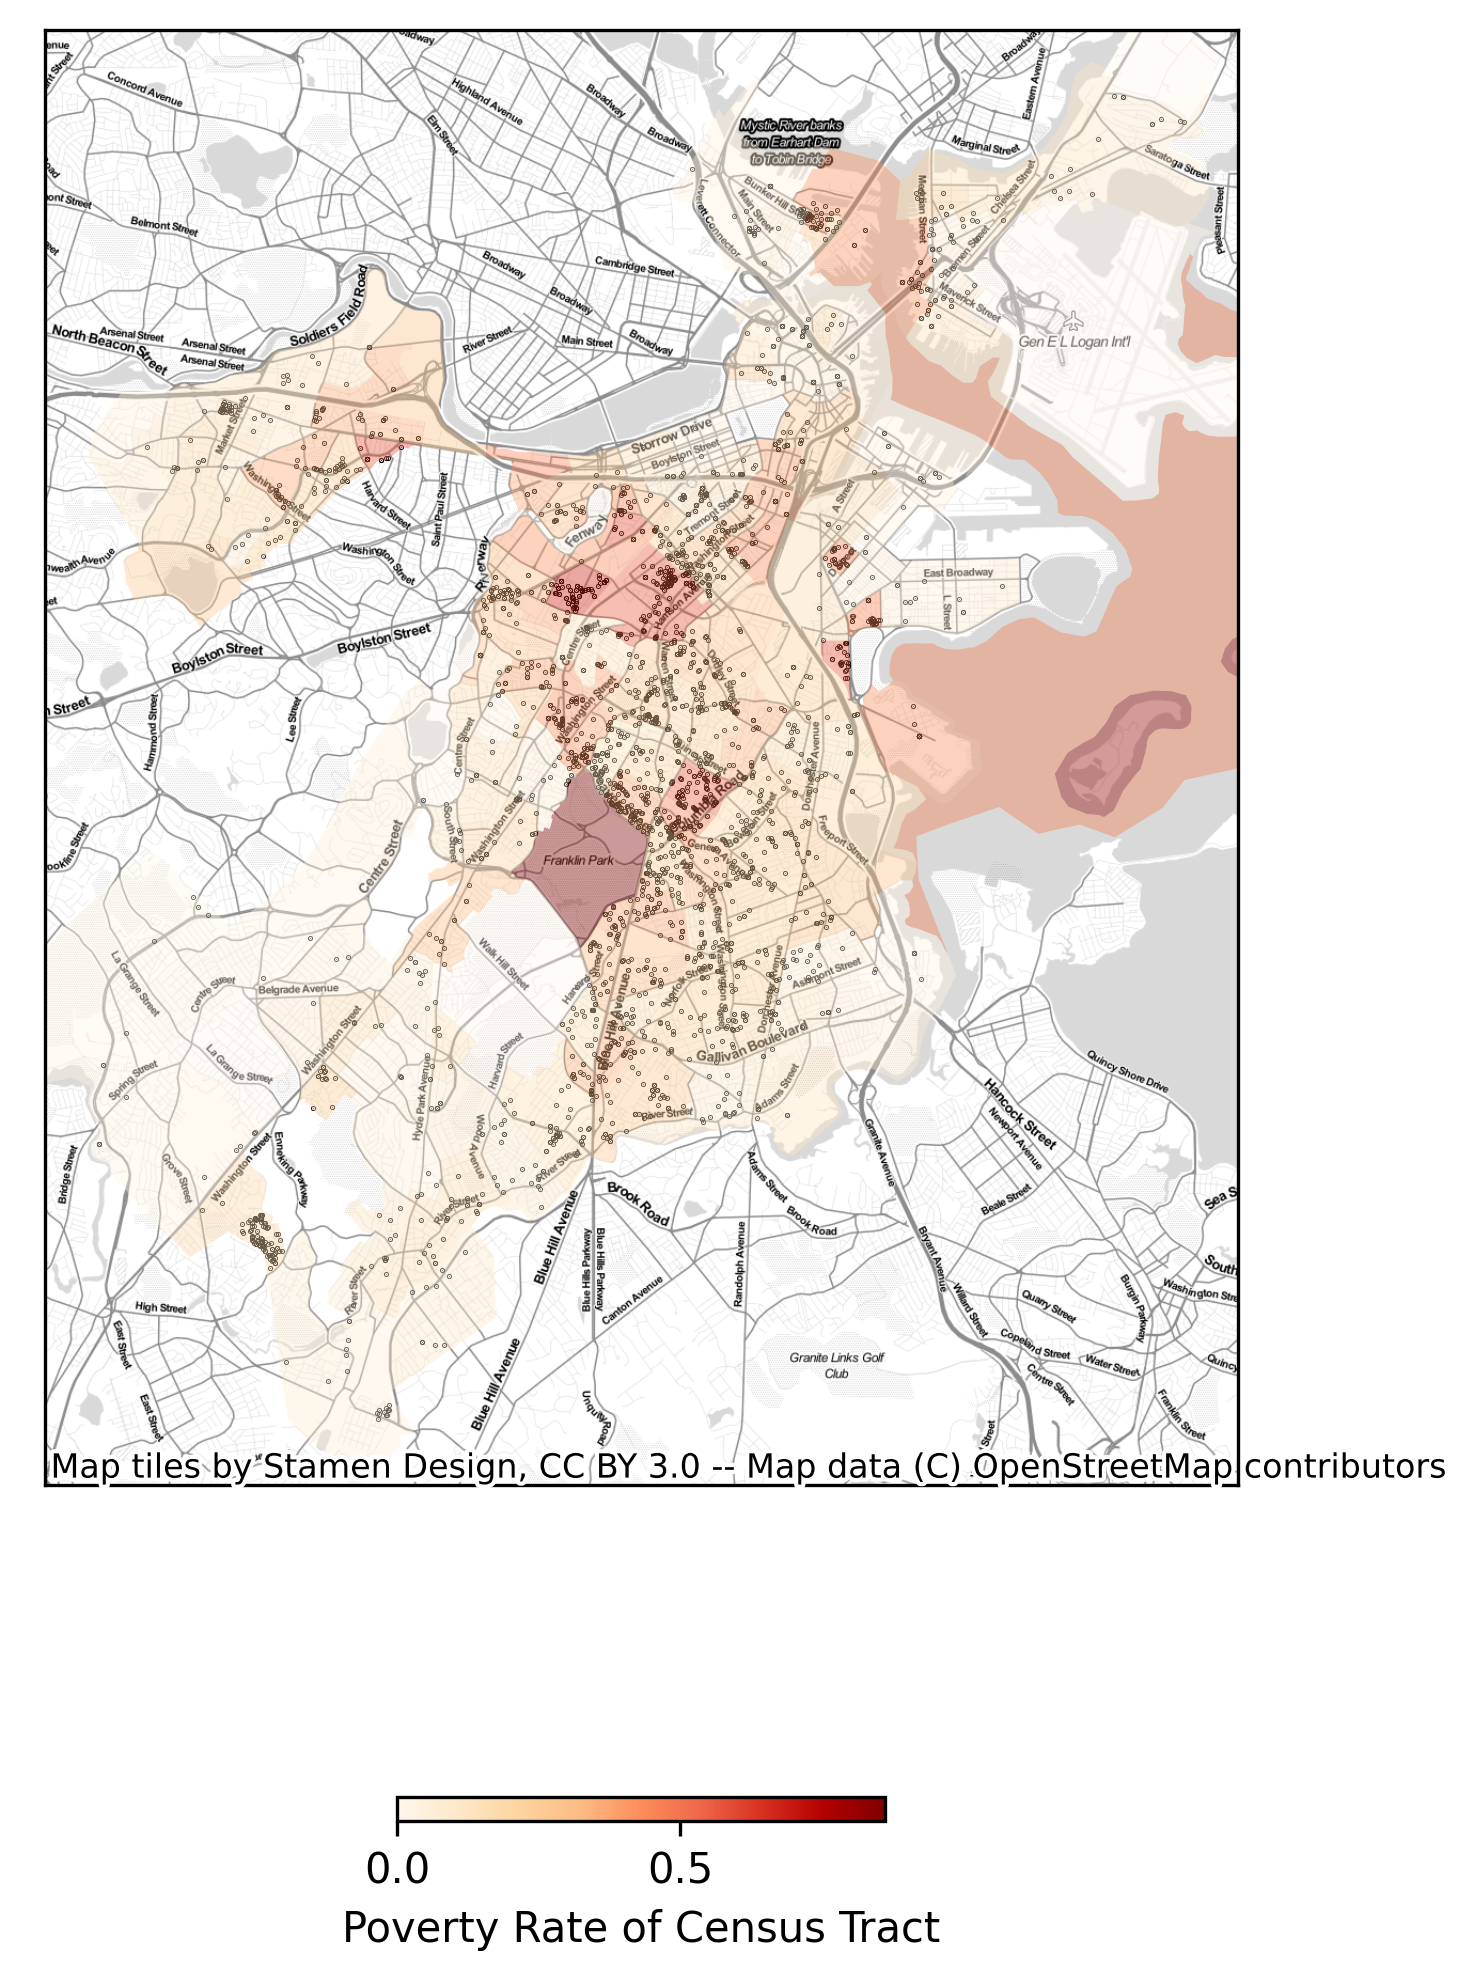
\includegraphics{output/summary_statistics/figures/evictions_map.png}
            \caption{Spatial Incidence of Eviction}
            \label{fig:my_label}
        \end{figure}

        \begin{figure}[H]
            \centering
            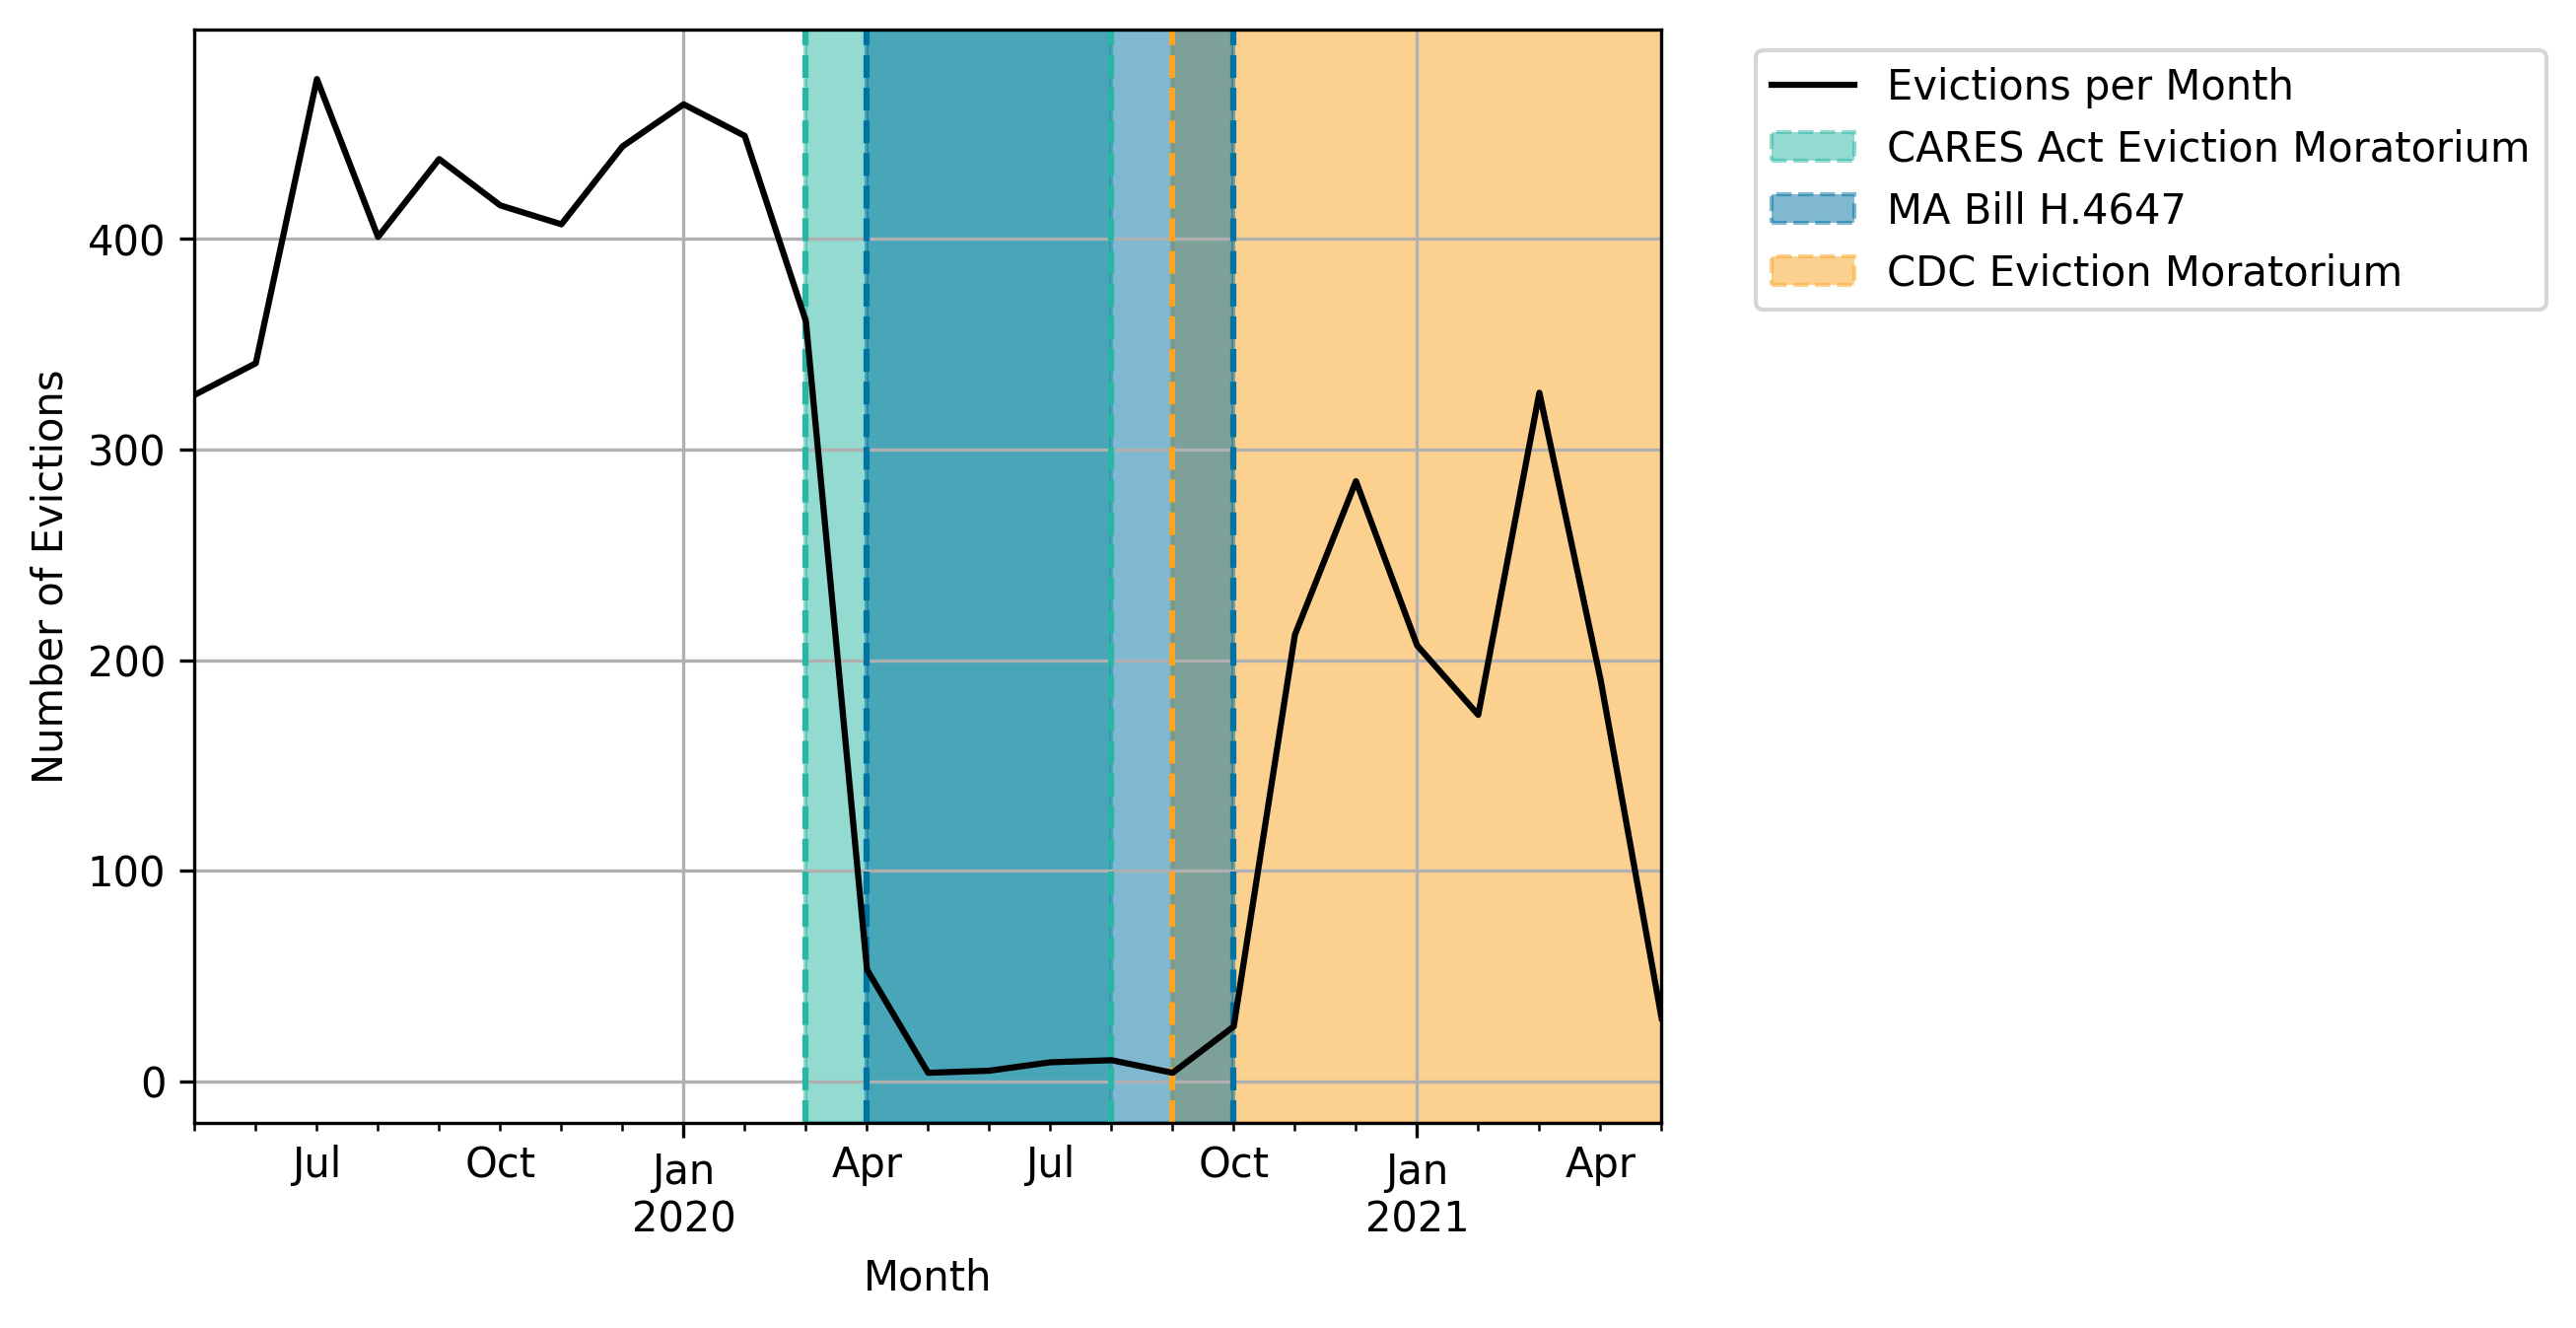
\includegraphics{output/summary_statistics/figures/filings_over_time.png}
            \caption{Eviction Filings Over Time}
            \label{fig:my_label}
        \end{figure}
    \end{landscape}
        \begin{table}[H]
            \centering
            \begin{tabular}{lccc}
\toprule
 & Cases Won By Defendant & Cases Won By Plaintiff & Portion of All Cases \\
\midrule
All Filing Dates & 858 & 2,440 & 1.00 \\
2019-05 & 100 & 156 & 0.08 \\
2019-06 & 38 & 151 & 0.06 \\
2019-07 & 42 & 198 & 0.07 \\
2019-08 & 31 & 178 & 0.06 \\
2019-09 & 37 & 156 & 0.06 \\
2019-10 & 33 & 148 & 0.05 \\
2019-11 & 23 & 138 & 0.05 \\
2019-12 & 28 & 171 & 0.06 \\
2020-01 & 17 & 159 & 0.05 \\
2020-02 & 38 & 139 & 0.05 \\
2020-03 & 70 & 85 & 0.05 \\
2020-04 & 14 & 19 & 0.01 \\
2020-05 & 0 & 1 & 0.00 \\
2020-06 & 2 & 2 & 0.00 \\
2020-07 & 1 & 2 & 0.00 \\
2020-08 & 1 & 2 & 0.00 \\
2020-09 & 1 & 6 & 0.00 \\
2020-10 & 7 & 14 & 0.01 \\
2020-11 & 54 & 151 & 0.06 \\
2020-12 & 71 & 159 & 0.07 \\
2021-01 & 81 & 120 & 0.06 \\
2021-02 & 58 & 86 & 0.04 \\
2021-03 & 58 & 89 & 0.04 \\
2021-04 & 45 & 93 & 0.04 \\
2021-05 & 8 & 17 & 0.01 \\
\bottomrule
\end{tabular}

            \caption{Distribution of Eviction Filings and Outcomes}
            \label{tab:my_label}
        \end{table}
    
    \subsection{Tax Assessment Records}
    \subsection{Zestimates}
        \begin{figure}[H]
            \centering
            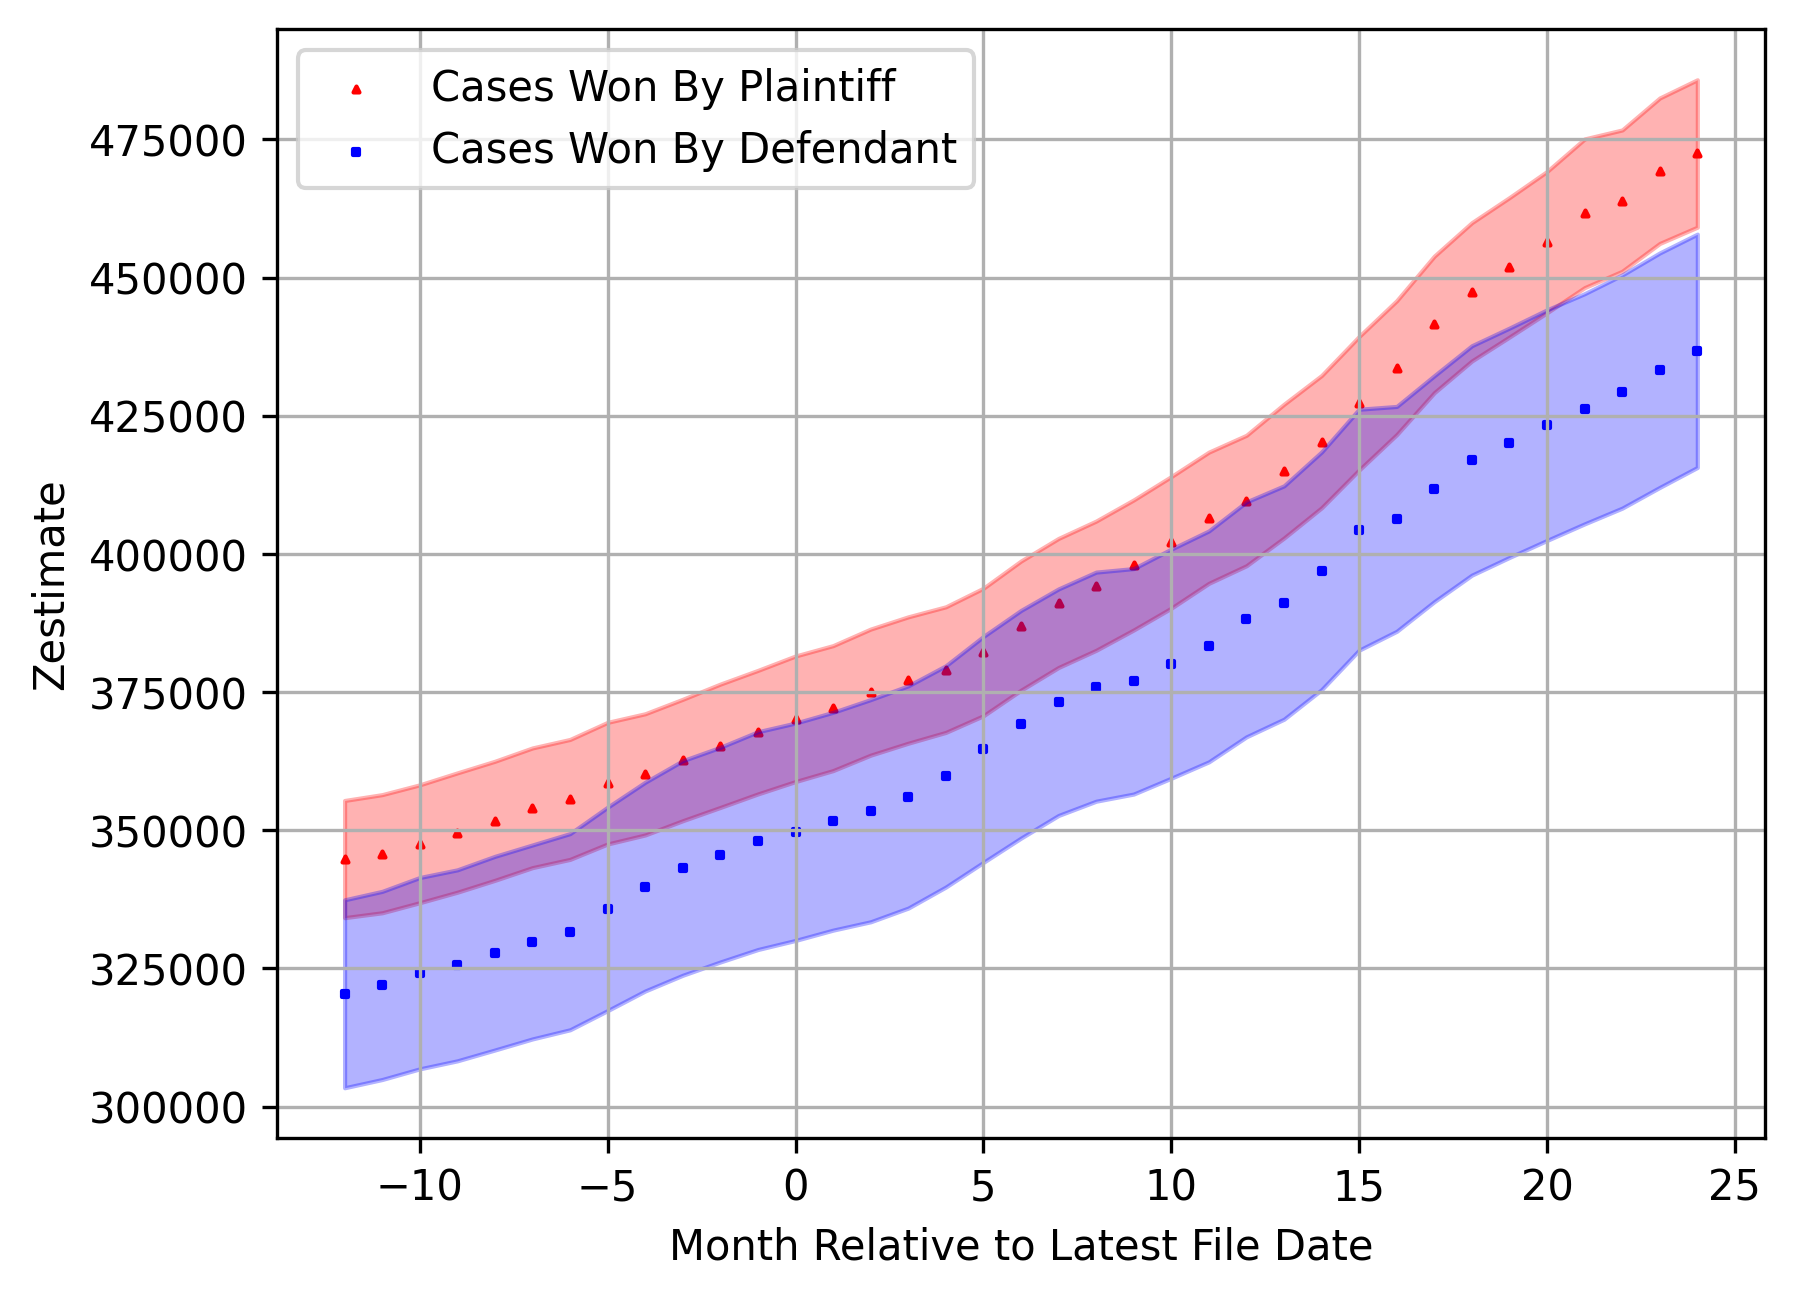
\includegraphics{output/summary_statistics/figures/trends_in_zestimates.png}
            \caption{Trends in Zestimates}
            \label{fig:my_label}
        \end{figure}

        \begin{figure}[H]
            \centering
            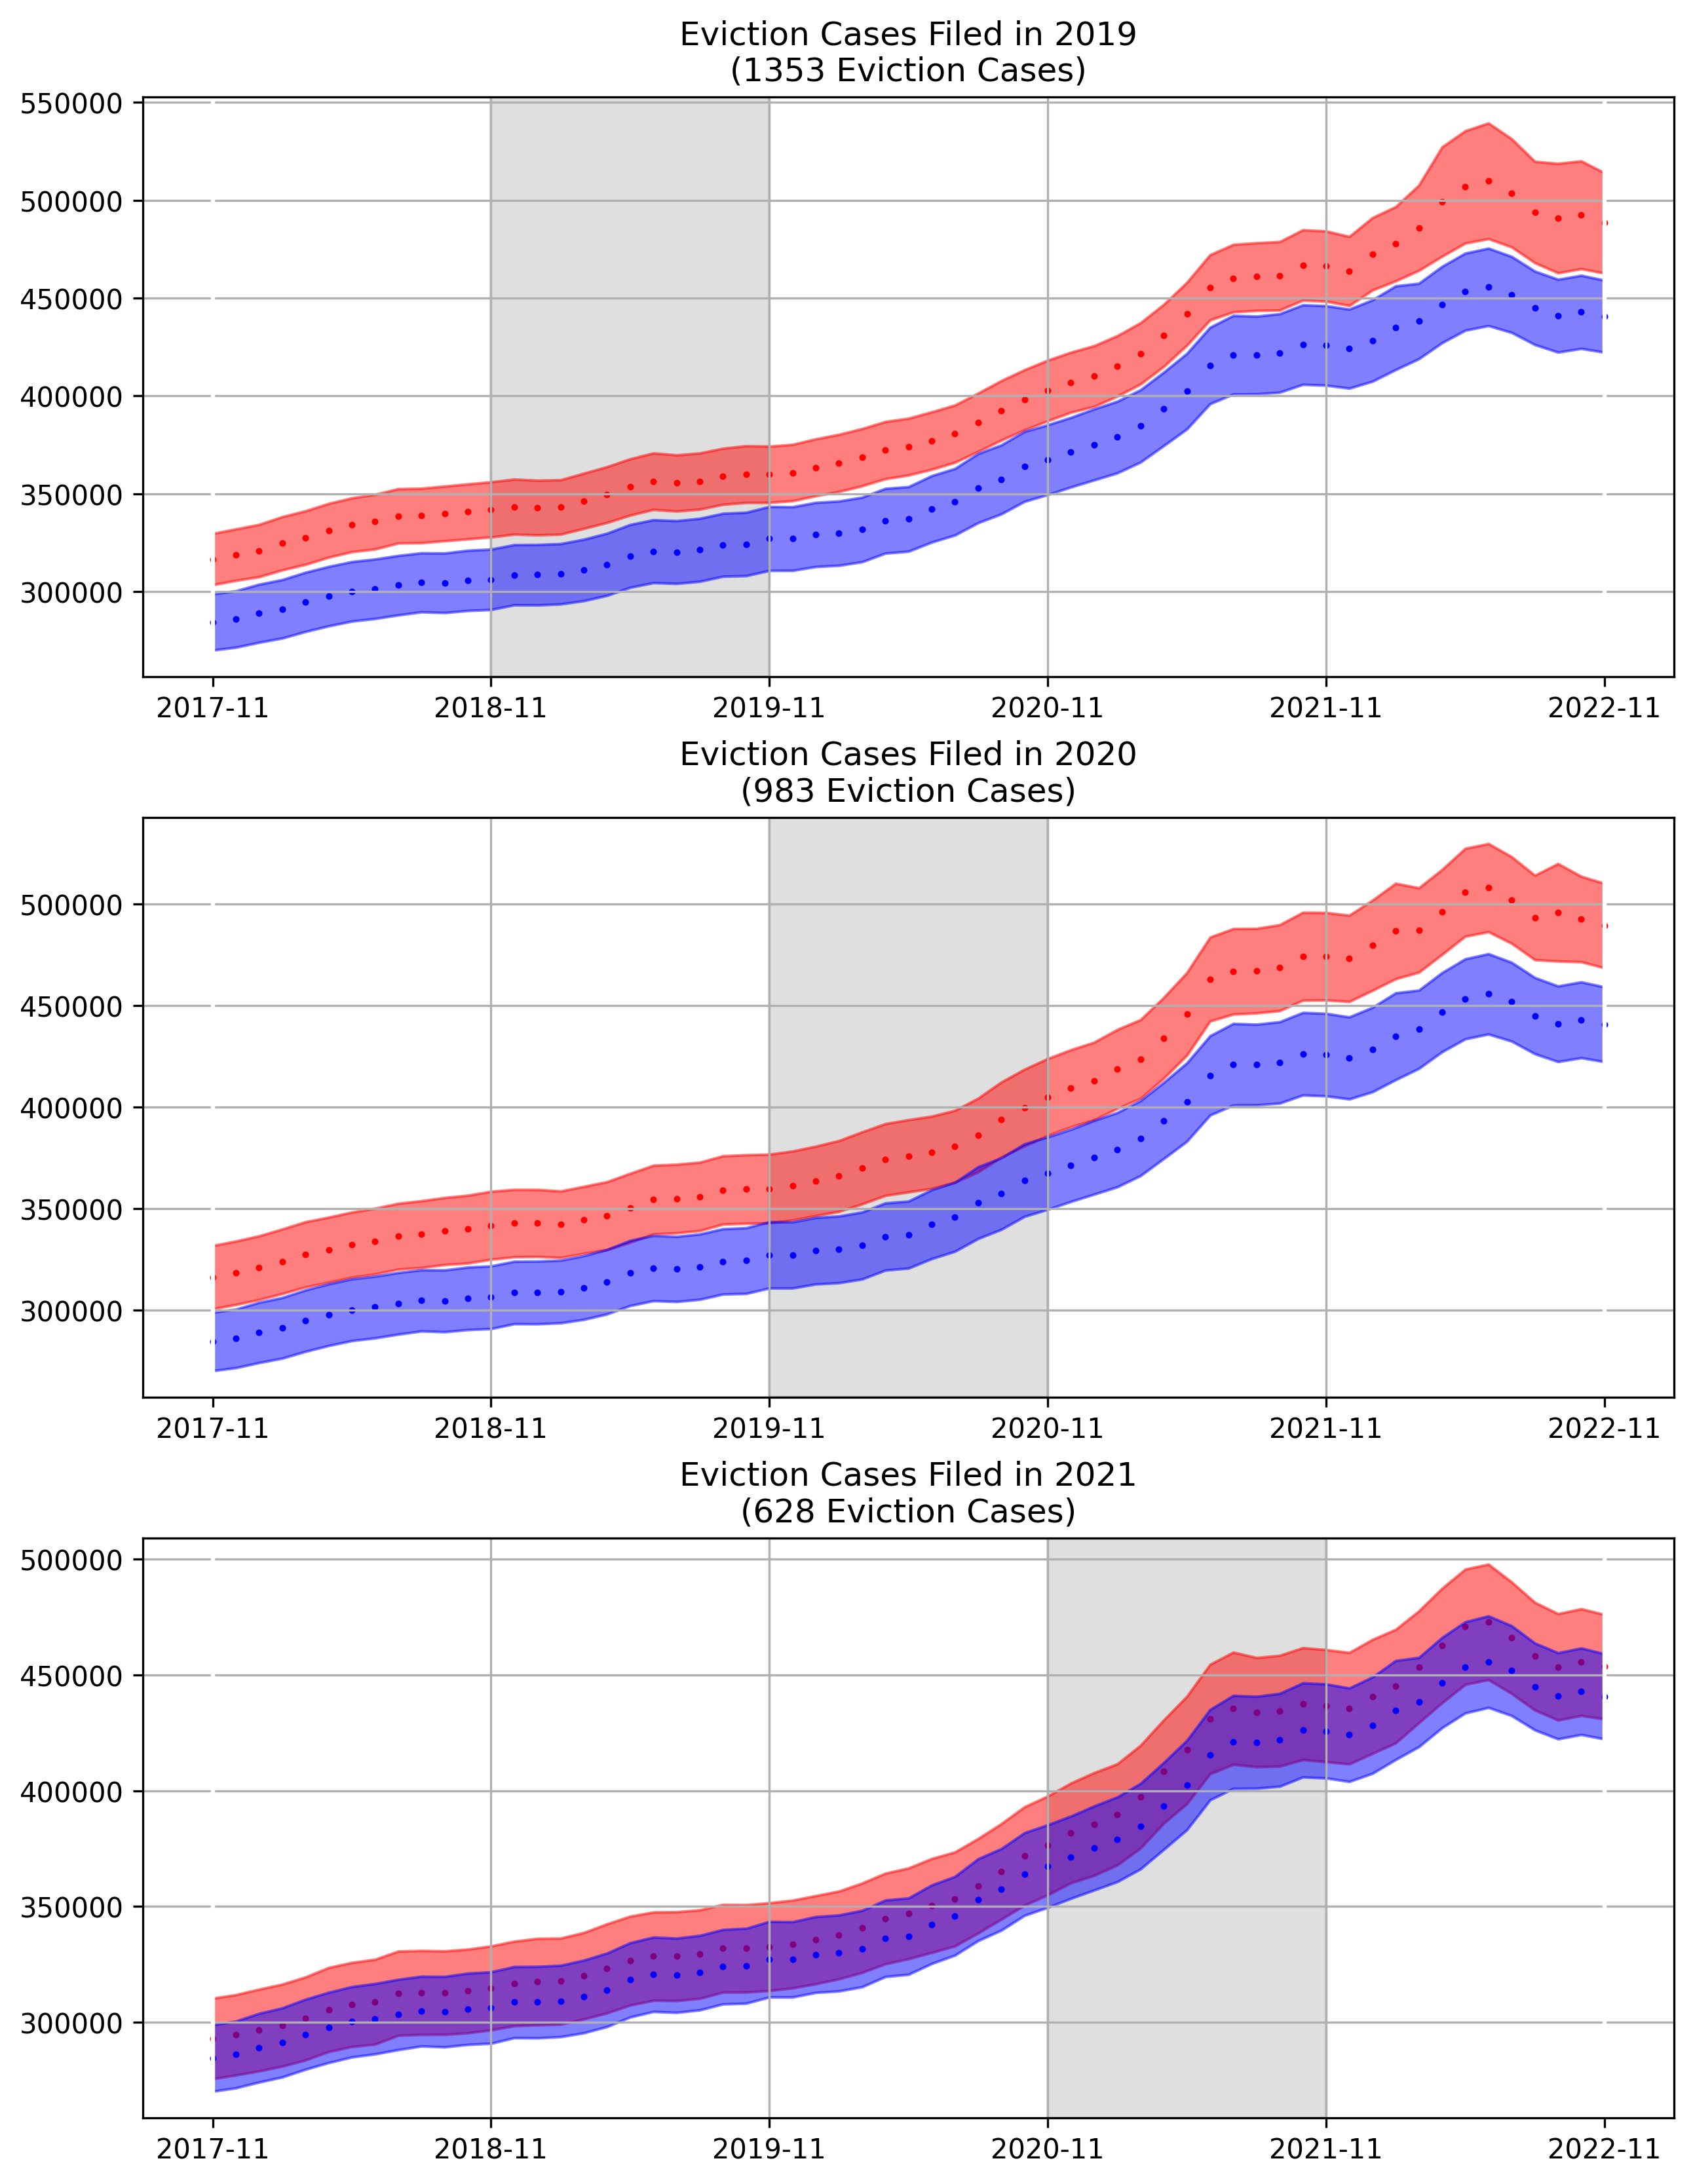
\includegraphics[scale=0.8]{output/DiD/figures/trends_in_zestimates_by_cohort.png}
            \caption{Trends in Zestimates by Cohort}
            \label{fig:my_label}
        \end{figure}

    \subsection{Summary Statistics}
         \begin{table}[H]
            \centering
            \small
            \begin{tabular}{llcccc}
\toprule
 &  & Mean & Median & S.D. & N \\
Panel & Variable &  &  &  &  \\
\midrule
\multirow[c]{3}{4cm}{\textit{Panel A: Case Initiation}} & For cause & 0.12 & 0.00 & 0.33 & 40,727 \\
 & No cause & 0.11 & 0.00 & 0.31 & 40,727 \\
 & Non-payment of rent & 0.75 & 1.00 & 0.43 & 40,727 \\
\cline{1-6}
\multirow[c]{6}{4cm}{\textit{Panel B: Case Resolution}} & Case defaulted & 0.20 & 0.00 & 0.40 & 40,727 \\
 & Case dismised & 0.29 & 0.00 & 0.45 & 40,727 \\
 & Case duration & 57.81 & 21.00 & 78.29 & 39,087 \\
 & Case heard & 0.06 & 0.00 & 0.23 & 40,727 \\
 & Case mediated & 0.41 & 0.00 & 0.49 & 40,727 \\
 & Money judgment & 1,890.34 & 0.00 & 5,279.49 & 40,727 \\
\cline{1-6}
\multirow[c]{4}{4cm}{\textit{Panel C: Defendant and Plaintiff Characteristics}} & Defendant has an attorney & 0.09 & 0.00 & 0.28 & 40,727 \\
 & Defendant is an entity & 0.01 & 0.00 & 0.08 & 40,727 \\
 & Plaintiff has an attorney & 0.84 & 1.00 & 0.37 & 40,727 \\
 & Plaintiff is an entity & 0.70 & 1.00 & 0.46 & 40,727 \\
\cline{1-6}
\multirow[c]{4}{4cm}{\textit{Panel D: Assessor Records From Most Recent Pre-Filing F.Y.}} & Building value & 8,350,204.19 & 636,500.00 & 22,073,916.94 & 36,587 \\
 & Land value & 2,471,065.61 & 192,400.00 & 6,218,383.08 & 36,587 \\
 & Other value & 112,575.80 & 1,000.00 & 659,661.29 & 36,587 \\
 & Total property value & 10,900,678.30 & 954,900.00 & 26,482,630.60 & 36,587 \\
\cline{1-6}
\multirow[c]{4}{4cm}{\textit{Panel E: Census Tract Characteristics}} & Median household income (2016) & 52,659.44 & 47,105.00 & 27,177.48 & 40,726 \\
 & Median two bedroom rent (2015) & 1,116.27 & 1,055.00 & 396.29 & 30,537 \\
 & Population density (2010) & 9,159.77 & 5,978.61 & 9,574.14 & 40,726 \\
 & Portion white (2010) & 0.58 & 0.63 & 0.29 & 40,726 \\
\cline{1-6}
\multirow[c]{9}{4cm}{\textit{Panel F: Zestimates Around Filing Date}} & Filing date & 377,384.02 & 305,144.00 & 316,645.29 & 10,096 \\
 & Five years before filing date & 261,462.86 & 213,270.60 & 238,040.64 & 9,842 \\
 & Four years before filing date & 280,243.32 & 225,065.75 & 276,051.45 & 9,968 \\
 & One year after filing date & 421,601.75 & 347,550.00 & 344,328.86 & 10,443 \\
 & One year before filing date & 351,172.05 & 278,722.25 & 311,982.74 & 10,190 \\
 & Three years after filing date & 501,611.80 & 414,600.00 & 780,467.01 & 5,894 \\
 & Three years before filing date & 307,137.16 & 240,097.38 & 369,763.53 & 10,172 \\
 & Two years after filing date & 477,948.08 & 393,900.00 & 457,694.83 & 9,175 \\
 & Two years before filing date & 341,084.08 & 259,176.00 & 987,145.51 & 10,182 \\
\cline{1-6}
\bottomrule
\end{tabular}

            \caption{Summary Statistics}
            \label{tab:table_1}
        \end{table}
        \newpage


    


\section{Empirical Strategy: Difference-in-Difference}
    I seek to estimate the average treatment effects of plaintiff victory in eviction cases on treated properties. I use the staggered difference-in-difference estimator proposed in \cite{callaway_difference--differences_2021}, which uses two-period, two-unit difference-in-difference estimators to estimate time- and cohort-specific ATTs and then aggregates them, weighting by cohort size, to produce summaries of the ATT. Let $G_i$ be the month during which the eviction case involving property $i$ was filed, such that $G_i = g \in \{\text{May} \; 2019, \text{June} \; 2019, ..., \text{May} \; 2021\}$. Let $C_i = 1$ if the eviction case involving $i$ resulted in a victory for the defendant and $0$ otherwise. If $G_i = g$ and $C_i = 0$, then property $i$ is a treated property and a member of the cohort first treated during month $g$. If $C_i=1$, then property $i$ is a never-treated property. 

    \subsection{Unconditional Estimates of the ATT}
    The following is an unconditional estimator for $ATT(g,t)$, the average treatment affect during month $t$ for the cohort first treated during month $g$.

    \begin{align}
        \hat{ATT}^{nev}_{un}(g, t) = \frac{\sum_i(Y_{i,t} - Y_{i, g-1})\mathds{1}\{G_i=g\}}{\sum_i\mathds{1}\{G_i=g\}} - \frac{\sum_i(Y_{i,t} - Y_{i, g-1})\mathds{1}\{C_i=1\}}{\sum_i\mathds{1}\{C_i=1\}}
    \end{align}

    This unconditional parallel trends assumption is unlikely to hold. Eviction case outcomes are likely to be endogenous to their socoioeconomic surroundings. Indeed, covariate exploration table reveals t

    \begin{table}[H]
        \tiny
        \centering
        \begin{tabular}{llcc}
\toprule
 &  & \multicolumn{2}{c}{\textit{Dependent Variable}} \\
\cline{3-4}
\\
 &  & Zestimate, Dec. 2022 & Plaintiff victory \\
 & \emph{Independent Variable} &  &  \\
\midrule
\multirow[c]{2}{3cm}{\textit{Panel A: Pre-treatment Zestimates}} & Zestimate, Jan. 2017 & 0.00 & 0.00 \\
 & Change, Jan. 2017 to Jan. 2019 & 0.00 & 0.27 \\
\cline{1-4}
\multirow[c]{8}{3cm}{\textit{Panel B: Census Tract Characteristics}} & Share with bachelor's degree & 0.00 & 0.07 \\
 & Jobs per square mile (2010) & 0.00 & 0.63 \\
 & Median household income (2016) & 0.00 & 0.01 \\
 & Share below poverty line & 0.70 & 0.01 \\
 & Population density (2010) & 0.00 & 0.01 \\
 & Median two bedroom rent (2015) & 0.00 & 0.05 \\
 & Share white (2010) & 0.00 & 0.00 \\
 & Share with commute $<$15 minutes (2010) & 0.00 & 0.02 \\
\cline{1-4}
\multirow[c]{3}{3cm}{\textit{Panel C: Case Initiation}} & For cause & 0.01 & 0.68 \\
 & No cause & 0.98 & 0.03 \\
 & Non-payment of rent & 0.31 & 0.77 \\
\cline{1-4}
\multirow[c]{4}{3cm}{\textit{Panel D: Defendant and Plaintiff Characteristics}} & Defendant has an attorney & 0.37 & 0.00 \\
 & Plaintiff has an attorney & 0.61 & 0.47 \\
 & Defendant is an entity & 0.02 & 0.37 \\
 & Plaintiff is an entity & 0.62 & 0.13 \\
\cline{1-4}
\bottomrule
\end{tabular}

        \caption{Caption}
        \label{tab:my_label}
    \end{table}


    \subsection{Estimating the ATT in the Staggered Treatment Case}
    I will use Callaway and Sant'Anna' (2021)'s multiperiod, staggered treatment difference-in-difference estimators. The following bullets summarize the empirical strategy informally; this information will eventually be placed appropriately into the subsection headers below this brief summary.
    \begin{enumerate}
        \item Reject conventional TWFE-DiD estimator. This estimator essentially estimates the ATT by performing a bunch of 2 unit, 2 period DiDs, then averages the calculated treatment effects. Goodman-Bacon (2021) shows that this estimator is composed in part of DiD estimates involving \emph{two units which are both treated during both periods}. This is in violation of the spirit of DiD. These incorrect DiD estimates are known as ``forbidden comparisons.''
        \item The way to properly recover the ATT is to basically perform all of the ``non-forbidden'' comparisons possible in our panel dataset. More formally:
        \begin{enumerate}
            \item We begin with a panel dataset of properties whose Zestimates are observed monthly. At each property $i$, an eviction case concludes during month $G_i=g$, resulting in a plaintiff victory or a defendant victory. These properties are collectively known as ``cohort $g$.'' If the eviction case at property $i$ resulted in a defendant victory, let $C_i=1$
            \item Break the units into ``cohorts'' according to the month in which their cases conclude. 
            \item We estimate $ATT(g, t)$, which is the average treatment effect on the treated for cohort $g$ at time $t$, by calculating the sample analog of:

            
            $E[Y_t - Y_{g-1}|G=g] - [Y_t - Y_{g-1}|C=1]$ 

            
            \item Intuitively, $ATT(g, t)$ comes from 2 period, 2 unit difference in difference estimate. The treatment group contains all units where we observe a plaintiff victory and the case was resolved at time $g$. The control group contains all units where we observe a defendant victory and the case was resolved at time $g$. We adjust the change in observed outcomes in the treatment group by the change in observed outcomes in the control group to get our estimate.
           
        \end{enumerate}
        \item The parallel trends and no anticipation assumptions are extended to the staggered treatment context.
            \begin{enumerate}
                \item \textbf{Staggered Treatment Adoption Assumption.} Let $D_it=1$ if unit $i$ has been treated by period $t$ and $D_it=0$ otherwise. Then, for $t=1,...,\tau$, $D_{it}=1 \rightarrow D_{it+1} = 1$. Basically, once a unit becomes treated, it stays treated.
                
                \item \textbf{Parallel Trends Assumption Based On Never Treated Units}. For all $g=2,...,\tau, t=2,...,\tau$ with $t\geq g$, we have

                $E[Y_t(0)-Y_{g-1}(0)|G=g]$ = $E[Y_t(0)-Y_{g-1}(0)|C=1]$

                Basically, for every possible 2 unit, 2 period DiD that we can run in our panel dataset between treated units and never-treated units, the canonical parallel trends assumption holds.
                
                
                \item \textbf{Parallel Trends Assumption Based On Not Yet Treated Units}. For all $g=2,...,\tau, s, t=2,...,\tau$ with $t \geq g$ and $s \geq t$, we have

                $E[Y_t(0) - Y_{t-1}(0)|G=g] = E[Y_t(0) - Y_{t-1}(0)|D_s=1, G \neq g]$

                This assumption allows us to use \emph{not yet treated} observations as a comparison group for \emph{treated} units. This is clearly a stronger assumption than the previous one and I have to think hard about whether I can make it in my case. Note that the graph in section 5.3 does NOT make this assumption.

                

                
            \end{enumerate}
        \item Now, we have a bunch of $ATT(g, t)$s. How do we aggregate them?
            \begin{enumerate}
                \item Take frequency-weighted averages across $t$ to get $ATT(g)$s, or ATTs for each cohort.
                \item Take frequency-weighted averages across $g$ to get $ATT(t)$s, or ATTs for each time period.
                \item Most convincing: calculate event time $e = t - g$. Now, $ATT(g, e_i)$ expresses the ATT on cohort $g$ at time relative to the end of the eviction case involving property $i$. Take frequency weighted averages across $g$ to get $ATT(e)s$, or ATTs for each period relative to the treatment period.
            \end{enumerate}
    \end{enumerate}

    \newpage
    \begin{landscape}
       \begin{table}[H]
        \centering
        \begin{tabular}{llccccc}
\toprule
 &  & \textit{} & \multicolumn{4}{c}{\textit{Difference in Cases Won by Defendant}} \\
\cline{4-7}
\\
 &  & Cases Won by Plaintiff & Unweighted & \emph{p} & Weighted & \emph{p} \\
\midrule
\multirow[c]{2}{3cm}{\textit{Panel A}} & Zestimate, Jan. 2017 & 291,945.81 & 26,673.96 & 0.00 & 3,189.17 & 0.75 \\
 & Change in Zestimate, Jan. 2017 to Jan. 2019 & 50,501.64 & 2,697.85 & 0.27 & -3,196.88 & 0.32 \\
\cline{1-7}
\multirow[c]{7}{3cm}{\textit{Panel B}} & Share with bachelor's degree & 0.25 & 0.01 & 0.09 & -0.00 & 0.96 \\
 & Jobs per square mile (2010) & 4,161.51 & 259.78 & 0.64 & 668.27 & 0.37 \\
 & Median household income (2016) & 52,084.78 & 2,271.04 & 0.03 & -211.14 & 0.87 \\
 & Population density (2010) & 9,018.27 & 962.56 & 0.01 & 644.23 & 0.17 \\
 & Median two bedroom rent (2015) & 1,093.52 & 33.19 & 0.05 & 8.19 & 0.69 \\
 & Share white (2010) & 0.60 & 0.03 & 0.00 & -0.00 & 0.94 \\
 & Share with commute $<$15 minutes (2010) & 0.29 & -0.01 & 0.02 & -0.01 & 0.29 \\
\cline{1-7}
\textit{Panel C} & For cause & 0.12 & 0.01 & 0.67 & -0.01 & 0.56 \\
\cline{1-7}
\textit{Panel D} & Defendant is an entity & 0.01 & 0.00 & 0.36 & 0.00 & 0.64 \\
\cline{1-7}
\bottomrule
\end{tabular}

        \caption{Caption}
        \label{tab:my_label}
    \end{table} 
    \end{landscape}
    
    \subsection{Parallel Trends Assumptions in the Staggered Treatment Case}
        
        \subsection{Testing Parallel Trends Empirically Using Rambachan and Roth (2022)}
    \subsection{Aggregating Treatment Effects Across Cohort and Time}
        \subsubsection{ATTs Across Cohorts}
        \subsubsection{ATTs Across Time Periods}
        \subsubsection{Event-Study ATTs}
    
\section{Results} \label{sec:result}
    \subsection{ATTs Across Cohorts}
    \subsection{ATTs Across Time Periods}
    \subsection{Event-Study ATTs}
        \begin{figure}[H]
            \centering
            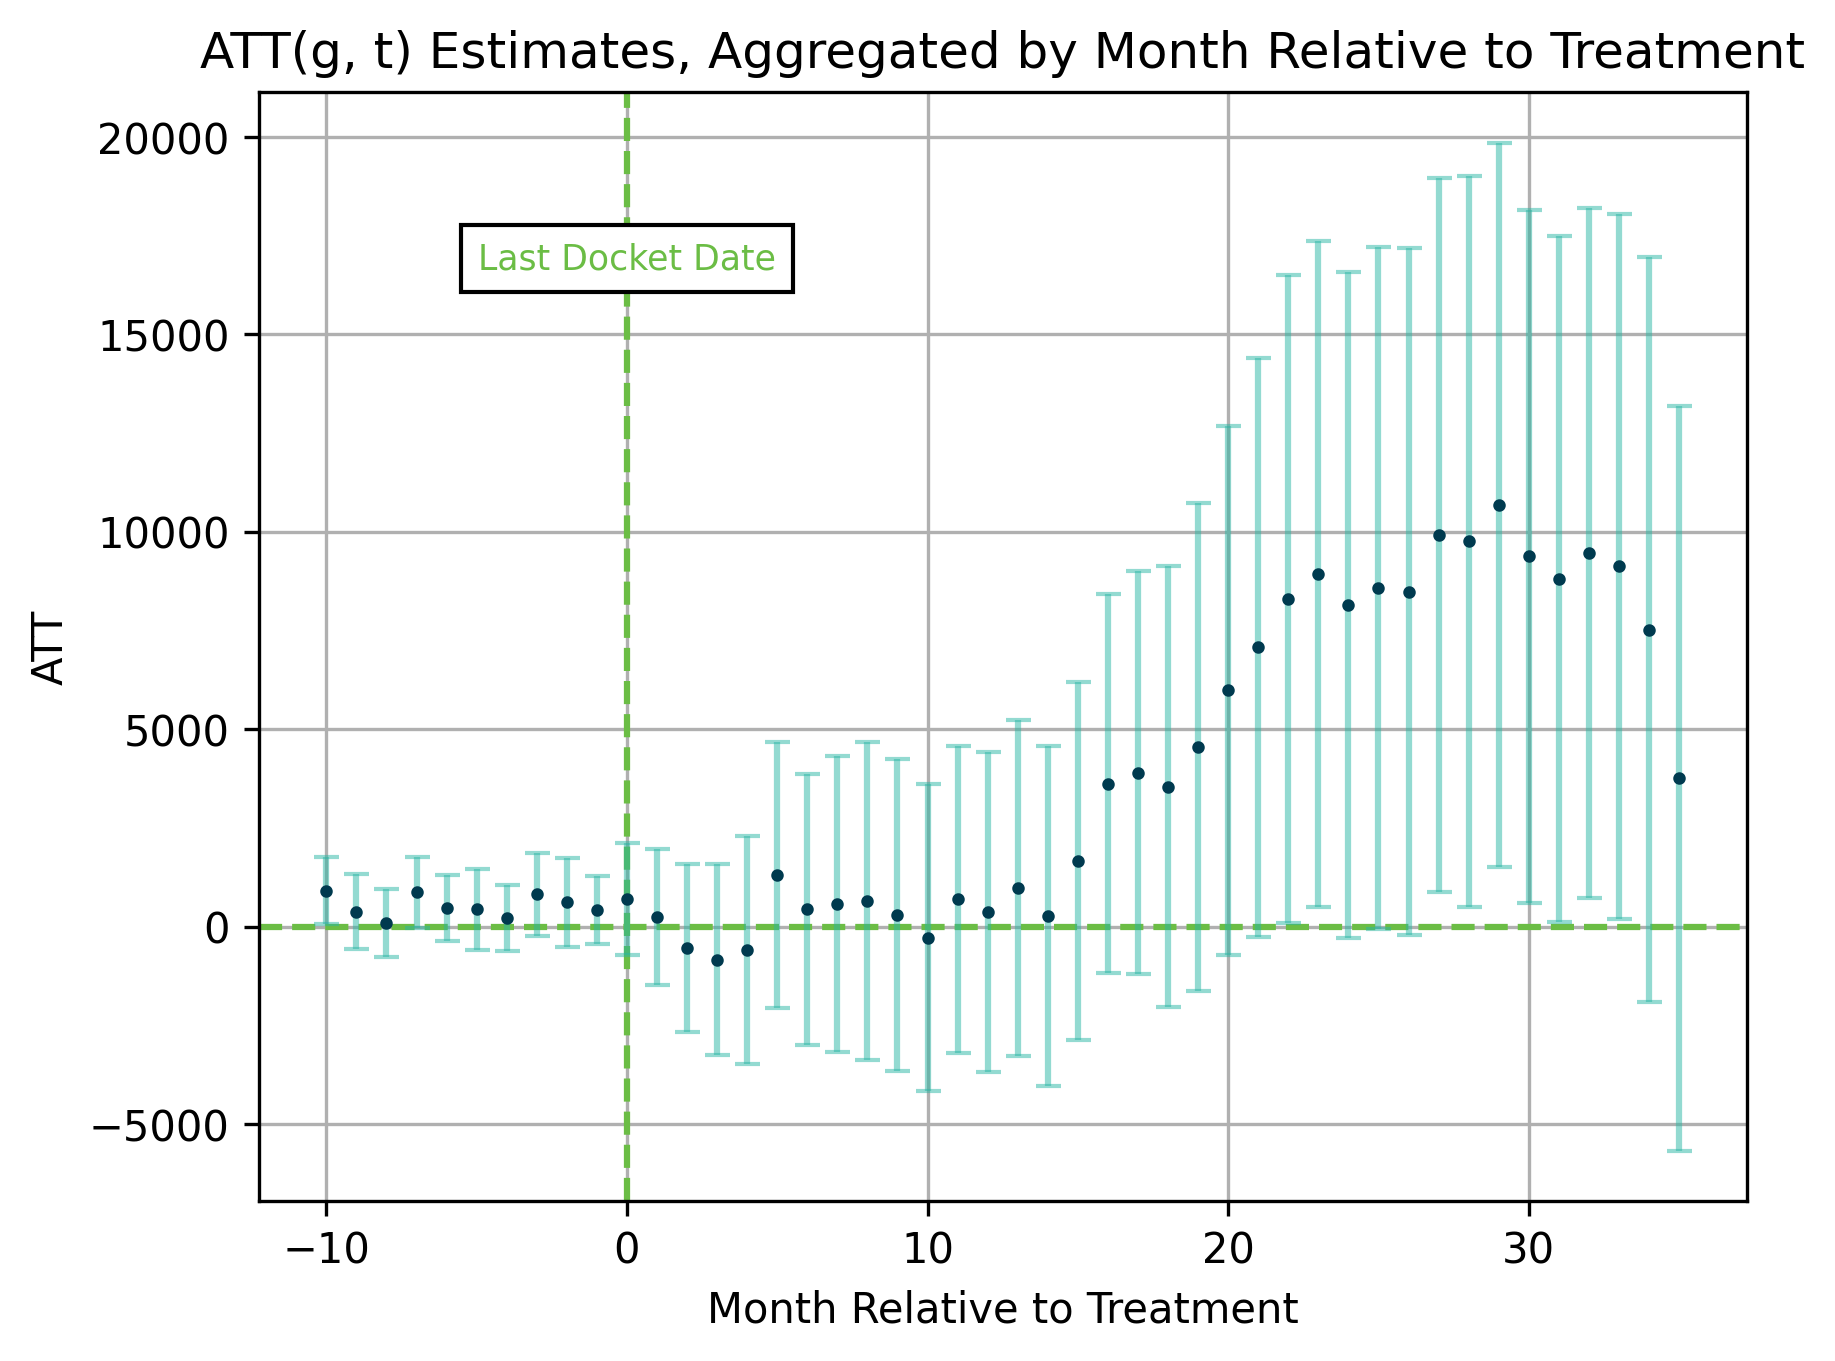
\includegraphics{output/DiD/figures/att_gt_estimates_event_study.png}
            \caption{$ATT(e)$s}
            \label{fig:my_label}
        \end{figure}


\section{Conclusion} \label{sec:conclusion}



\clearpage

\onehalfspacing

%
\end{document}